\documentclass[12pt]{article}
\usepackage[margin=1in]{geometry}
\usepackage{listings}
\usepackage{graphicx}
\usepackage{float}
\usepackage{color} %red, green, blue, yellow, cyan, magenta, black, white
\definecolor{mygreen}{RGB}{28,172,0} % color values Red, Green, Blue
\definecolor{mylilas}{RGB}{170,55,241}

\setlength{\parskip}{1em}

\lstset{language=Matlab,%
    %basicstyle=\color{red},
    breaklines=true,%
    morekeywords={matlab2tikz},
    keywordstyle=\color{blue},%
    morekeywords=[2]{1}, keywordstyle=[2]{\color{black}},
    identifierstyle=\color{black},%
    stringstyle=\color{mylilas},
    commentstyle=\color{mygreen},%
    showstringspaces=false,%without this there will be a symbol in the places where there is a space
    numbers=left,%
    numberstyle={\tiny \color{black}},% size of the numbers
    numbersep=9pt, % this defines how far the numbers are from the text
    emph=[1]{for,end,break},emphstyle=[1]\color{red}, %some words to emphasise
    %emph=[2]{word1,word2}, emphstyle=[2]{style},    
}

\usepackage{mathtools}
\usepackage{url}

\title{Assignment 4, COMP4702}
\author{Roy Portas, 43560846}
\date{\today}

\begin{document} 
\begin{titlepage}
    \maketitle
\end{titlepage}

\section*{Prac 10}

\subsection*{Question 3}

\begin{figure}[H]
    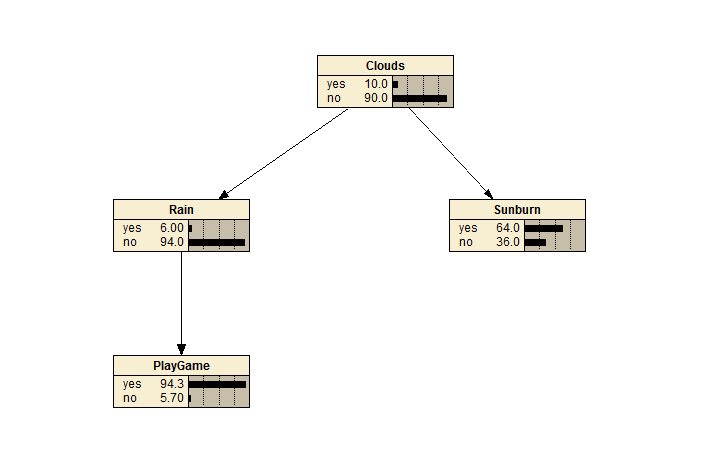
\includegraphics[width=\linewidth]{../../pracs/prac10/q3_network}
    \centering
    \caption{Network}
\end{figure}

The probabilities in the network match the course notes, thus are valid.

\begin{figure}[H]
    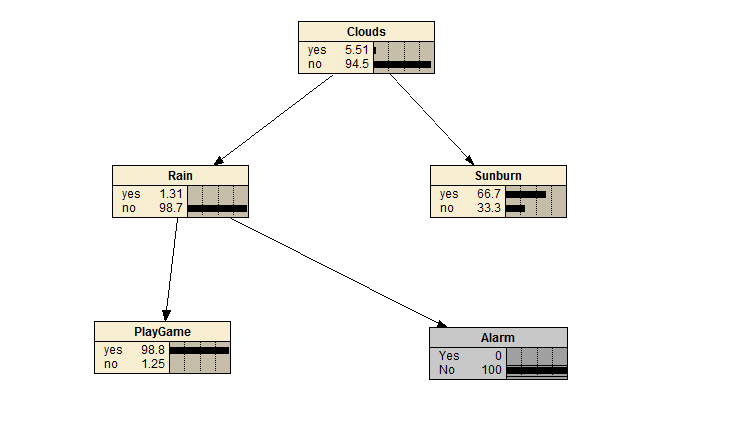
\includegraphics[width=\linewidth]{../../pracs/prac10/q3_no_rain}
    \centering
    \caption{No Rain}
\end{figure}

If there is no rain then the chance of clouds decrease by around a half, to 4.26\%.
Since it is not raining, there is a 100\% chance the game will be played.
Additionally the chance of sunburn increases by around 3\%.

\subsection*{Question 4}



\begin{figure}[H]
    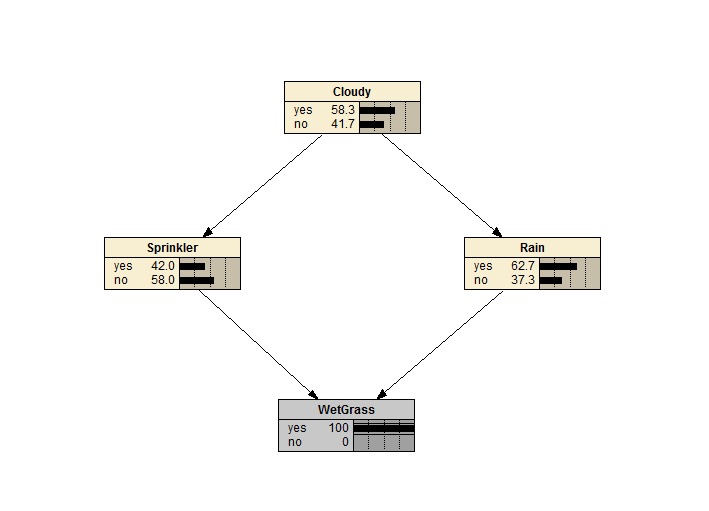
\includegraphics[width=\linewidth]{../../pracs/prac10/q4}
    \centering
    \caption{Network}
\end{figure}

\section*{Prac 11}

\subsection{Question 1}

\lstinputlisting[language=Matlab]{../../pracs/prac11/q1.m}

\begin{figure}[H]
    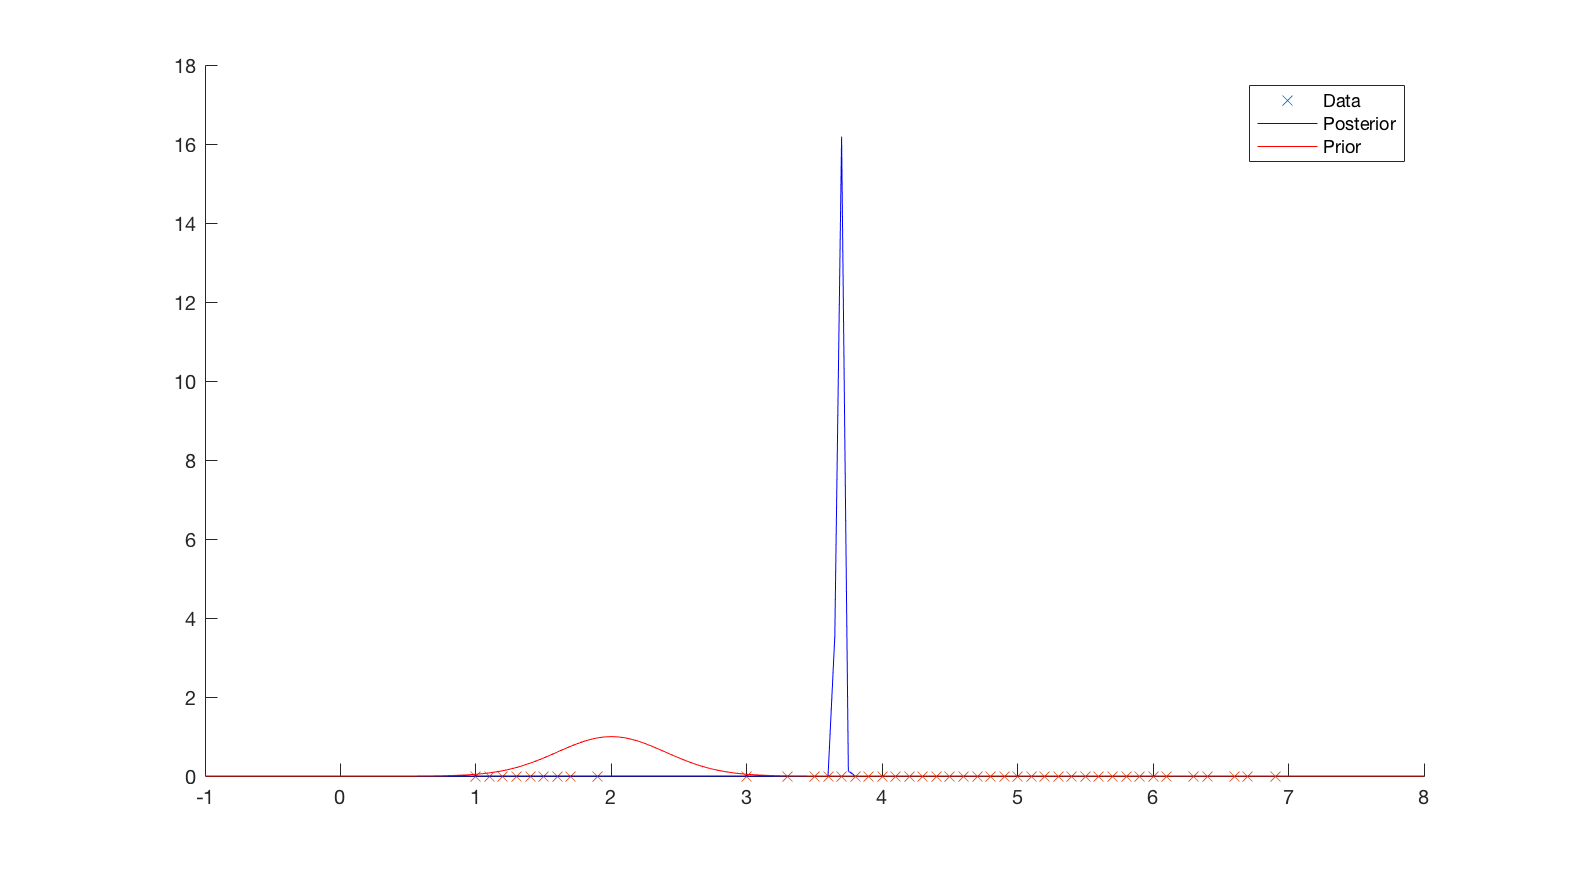
\includegraphics[width=\linewidth]{../../pracs/prac11/q1_graph}
    \centering
    \caption{Model prior and posterior distributions}
\end{figure}

\end{document}
